\section{Subroutines and Stack}

\subsubsection{Subroutine}

\begin{concept}{Subroutine Basics}\\
Key elements of subroutines:
\begin{itemize}
  \item Label to identify subroutine entry point
  \item Return instruction (BX LR) to exit
  \item Proper register management
\end{itemize}
\end{concept}

\begin{example2}{Subroutine Call and Return}\\
Multiply by 3 implementation:
\begin{lstlisting}[language=armasm, style=basesmol]
MulBy3  MOV     R4, R0      ; Save input value
        LSLS    R0, #1      ; Multiply by 2
        ADD     R0, R4      ; Add original value
        BX      LR          ; Return
\end{lstlisting}

in detail:
\begin{itemize}
  \item Label with name \textcolor{darkred}{\textbf{MulBy3}}
  \item Return Statement \textcolor{darkblue}{\textbf{BX LR}}
\end{itemize}

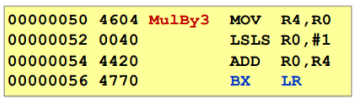
\includegraphics[width=0.7\linewidth]{images/subroutine.png}
\end{example2}

\begin{concept}{Call and Return Mechanism}\\
Basic subroutine mechanics:
\begin{itemize}
  \item \textbf{BL (Branch with Link)}:
    \begin{itemize}
      \item Stores current PC in LR (R14)
      \item Branches to subroutine address
      \item Direct and relative addressing
    \end{itemize}
  \item \textbf{BLX (Branch with Link and Exchange)}:
    \begin{itemize}
      \item Similar to BL but with register-specified target
      \item Indirect and absolute addressing
    \end{itemize}
  \item \textbf{Return}:
    \begin{itemize}
      \item Using BX LR
      \item Or POP {..., PC} if LR was saved
    \end{itemize}
\end{itemize}
\end{concept}

\begin{example2}{Nested Subroutine Calls}
Example of nested calls:
\begin{lstlisting}[language=armasm, style=basesmol]
main
    BL      proc_a          ; Call proc_a
    ; continue main
    
proc_a
    PUSH    {LR}            ; Save return address
    BL      proc_b          ; Call proc_b
    POP     {PC}            ; Return to main
    
proc_b
    PUSH    {LR}            ; Save return address
    BL      proc_c          ; Call proc_c
    POP     {PC}            ; Return to proc_a
    
proc_c
    ; Do something
    BX      LR              ; Return to proc_b
\end{lstlisting}
\end{example2}

\subsubsection{Stack}

\begin{definition}{Stack}characteristics:
\begin{itemize}
  \item \textcolor{darkblue}{\textbf{Stack Area}} (Section): Continuous RAM section
  \item \textcolor{darkred}{\textbf{Stack Pointer (SP)}}: R13, points to last written value
  \item \textbf{Direction}: Full-descending (grows toward lower addresses)
  \item \textbf{Alignment}: Word-aligned (4 bytes)
  \item \textbf{Data Size}: 32-bit words only
\end{itemize}

Main operations:
\begin{itemize}
  \item \textcolor{darkgreen}{\textbf{PUSH}}: Decrements SP, then stores words
  \item \textcolor{darkgreen}{\textbf{POP}}: Loads words, then increments SP
\end{itemize}

Stack constraints:
\begin{itemize}
  \item Number of PUSH and POP operations must match
  \item SP must stay between stack-limit and stack-base\\
  $\rightarrow$ \textcolor{darkgreen}{Stack-limit} $\leq$ SP $\leq$ \textcolor{darkpurple}{Stack-base}
\end{itemize}

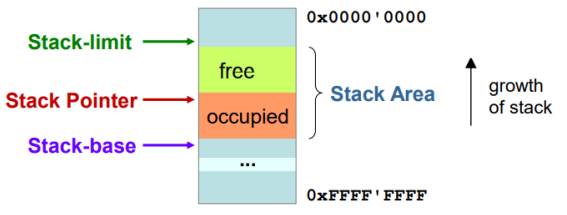
\includegraphics[width=\linewidth]{images/stack_overview.png}


\end{definition}

\begin{concept}{Stack Instructions}

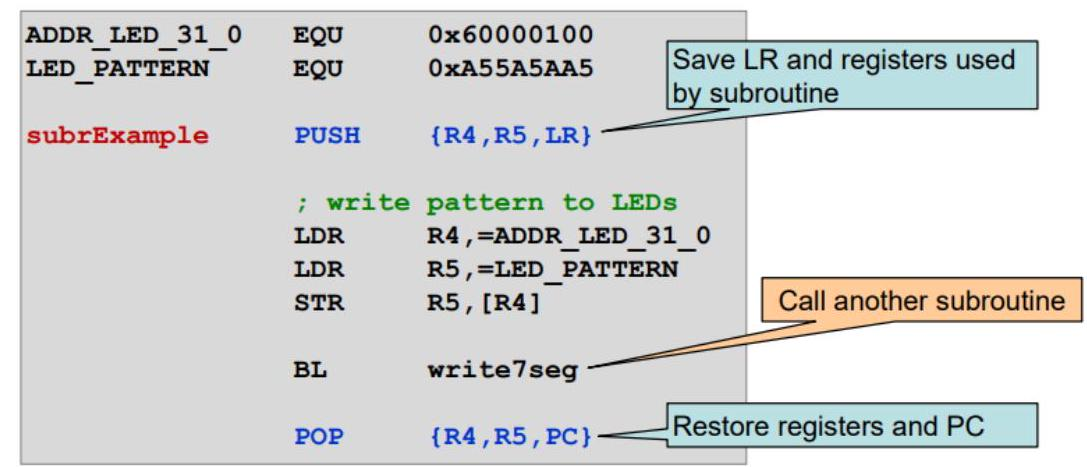
\includegraphics[width=\linewidth]{images/2024_12_29_79e6b22f503fb7b4f718g-08}


Special stack manipulation instructions:
\vspace{1mm}\\
\begin{minipage}[t]{0.5\linewidth}
\begin{itemize}
  \item \textbf{ADD/SUB SP}:
    \begin{itemize}
      \item Immediate offset 0-508
      \item Must be multiple of 4
    \end{itemize}
  \item \textbf{SP-relative LDR/STR}:
    \begin{itemize}
      \item Immediate offset 0-1020
      \item Used for frame access
    \end{itemize}
\end{itemize}
\end{minipage}
\begin{minipage}[t]{0.5\linewidth}
\begin{itemize}
  \item \textbf{PUSH/POP}:
    \begin{itemize}
      \item Multiple register transfer
      \item Maintains alignment
      \item Can include PC/LR
    \end{itemize}
\end{itemize}
\end{minipage}
\end{concept}

\begin{example2}{PUSH/POP Implementation}
\begin{lstlisting}[language=armasm, style=basesmol]
    ; PUSH {R2,R3,R6}
    SUB     SP, SP, #12     ; Reserve stack space
    STR     R2, [SP]        ; Store R2
    STR     R3, [SP, #4]    ; Store R3
    STR     R6, [SP, #8]    ; Store R6

    ; POP {R2,R3,R6}
    LDR     R2, [SP]        ; Restore R2
    LDR     R3, [SP, #4]    ; Restore R3
    LDR     R6, [SP, #8]    ; Restore R6
    ADD     SP, SP, #12     ; Free stack space
\end{lstlisting}
\end{example2}





\begin{definition}{Stack Frame Structure}\\
Components of a stack frame:
\begin{itemize}
  \item \textbf{Saved Registers}:
    \begin{itemize}
      \item Caller-saved (R0-R3, R12)
      \item Callee-saved (R4-R11)
      \item Link register (LR)
    \end{itemize}
  \item \textbf{Local Variables}:
    \begin{itemize}
      \item Allocated on stack if needed
      \item Word-aligned access
    \end{itemize}
  \item \textbf{Parameters}:
    \begin{itemize}
      \item Beyond R0-R3 if needed
      \item Pushed by caller
    \end{itemize}
\end{itemize}

%\includegraphics[width=\linewidth]{images/2024_12_29_79e6b22f503fb7b4f718g-08(1)}
\end{definition}

\begin{KR}{Stack Frame Management}\\
Steps for function prologue and epilogue:

1. Function Prologue:
\begin{lstlisting}[language=armasm, style=basesmol]
    PUSH    {R4-R7, LR}     ; Save registers
    SUB     SP, SP, #locals ; Allocate local vars
\end{lstlisting}

2. Function Epilogue:
\begin{lstlisting}[language=armasm, style=basesmol]
    ADD     SP, SP, #locals ; Deallocate locals
    POP     {R4-R7, PC}     ; Restore and return
\end{lstlisting}

3. Stack frame access:
\begin{lstlisting}[language=armasm, style=basesmol]
    ; Access local variables
    STR     R0, [SP, #0]    ; First local
    STR     R1, [SP, #4]    ; Second local
    
    ; Access parameters
    LDR     R0, [SP, #20]   ; First stack parameter
\end{lstlisting}
\end{KR}

\begin{example2}{Stack Frame Layout}
Example of complete function:
\begin{lstlisting}[language=armasm, style=basesmol]
; int calc(int a, int b, int c)
; a in R0, b in R1, c in R2
calc    PUSH    {R4-R6, LR} ; Save registers
        
        ; Save parameters
        MOVS    R4, R0      ; Save a
        MOVS    R5, R1      ; Save b
        MOVS    R6, R2      ; Save c
        
        ; Call helper function
        MOVS    R0, R4      ; First param
        BL      helper      ; Call helper
        
        ; Continue calculation
        ADDS    R0, R5      ; Add b
        ADDS    R0, R6      ; Add c
        
        POP     {R4-R6, PC} ; Return
\end{lstlisting}
\end{example2}

\begin{remark}
Stack usage considerations:
\begin{itemize}
  \item Monitor stack depth in nested calls
  \item Always maintain 8-byte alignment for SP
  \item Consider register usage to minimize stack operations
  \item Be aware of stack space in interrupt handlers
  \item Document stack requirements for functions
\end{itemize}
\end{remark}

\begin{KR}{Using Subroutines and Stack}\\
Steps for implementing subroutines:
\begin{enumerate}
  \item Define subroutine entry point with label
  \item Save registers that will be modified
    \begin{itemize}
      \item Use PUSH at start
      \item Include LR if calling other subroutines
    \end{itemize}
  \item Implement subroutine logic
  \item Restore registers in reverse order
    \begin{itemize}
      \item Use POP before return
      \item Can return using POP {..., PC} if LR was saved
    \end{itemize}
  \item Return using BX LR if LR wasn't saved
\end{enumerate}
\end{KR}

\begin{remark}
Important considerations:
\begin{itemize}
  \item Always maintain stack alignment
  \item Match PUSH/POP pairs exactly
  \item Be careful with SP manipulation
  \item Consider nesting depth for stack space
\end{itemize}
\end{remark}

\begin{KR}{Function Implementation Patterns}\\
Common implementation patterns:

1. Simple function:
\begin{lstlisting}[language=armasm, style=basesmol]
func    PUSH    {LR}        ; Save return address
        ; Function body
        POP     {PC}        ; Return
\end{lstlisting}

2. Function with locals:
\begin{lstlisting}[language=armasm, style=basesmol]
func    PUSH    {R4, LR}    ; Save registers
        SUB     SP, #8      ; Space for locals
        ; Function body
        ADD     SP, #8      ; Remove locals
        POP     {R4, PC}    ; Return
\end{lstlisting}

3. Function with parameters:
\begin{lstlisting}[language=armasm, style=basesmol]
        ; R0-R3 = first 4 parameters
        ; [SP] = fifth parameter
func    PUSH    {R4-R6, LR} ; Save registers
        LDR     R4, [SP, #16] ; Load 5th param
        ; Function body
        POP     {R4-R6, PC} ; Return
\end{lstlisting}
\end{KR}



